% !TEX root = ../thesis-main.tex

\section{Discussion}
\label{section:6}
Since our original motivation was to provide an explanation system that can be used by forecasting analysts, we conducted a more in-depth analysis of the results to determine if there was a difference in attitudes between users depending on their background (e.g., practitioners from \OurCompany{} or researchers from the university). 




\subsection{Comparing Attitudes Conditioned on Background}
\label{section:conditioning}
Table~\ref{table:background} shows the distribution of practitioners and researchers in the treatment and control groups. 
Since we have a slight imbalance in background between the treatment and control groups, we test whether or not our results still hold when conditioning on background and confirm that they do. 



Again, we do not find statistically significant differences in initial attitudes towards the model ($\chi^{2}$ test, $\alpha = 0.05$). 
For researchers, the distribution of answers between treatment and control groups is significantly different for SQ1 ($\chi^{2} = 14.2$, $\alpha = 0.001$), but does not differ for SQ2, SQ3, or SQ4 ($\chi^{2}$ test, $\alpha = 0.05$). 
The same holds for practitioners: the distributions are significantly different only for SQ1 ($\chi^{2} = 6.94$, $\alpha = 0.05$). 
This is consistent with our results in Section~\ref{section:5}. 
In both cases, users in the treatment group agree with SQ1 more than users in the control group, indicating that \OurMethod{} explanations help users understand why the model makes large errors in predictions, regardless of whether they are practitioners or researchers.  
Although the results are statistically significant for both groups, it should be noted that the results hold more strongly for researchers compared to those for practitioners, given the $\chi^{2}$ values. 

\begin{figure}[t]
 \centering
 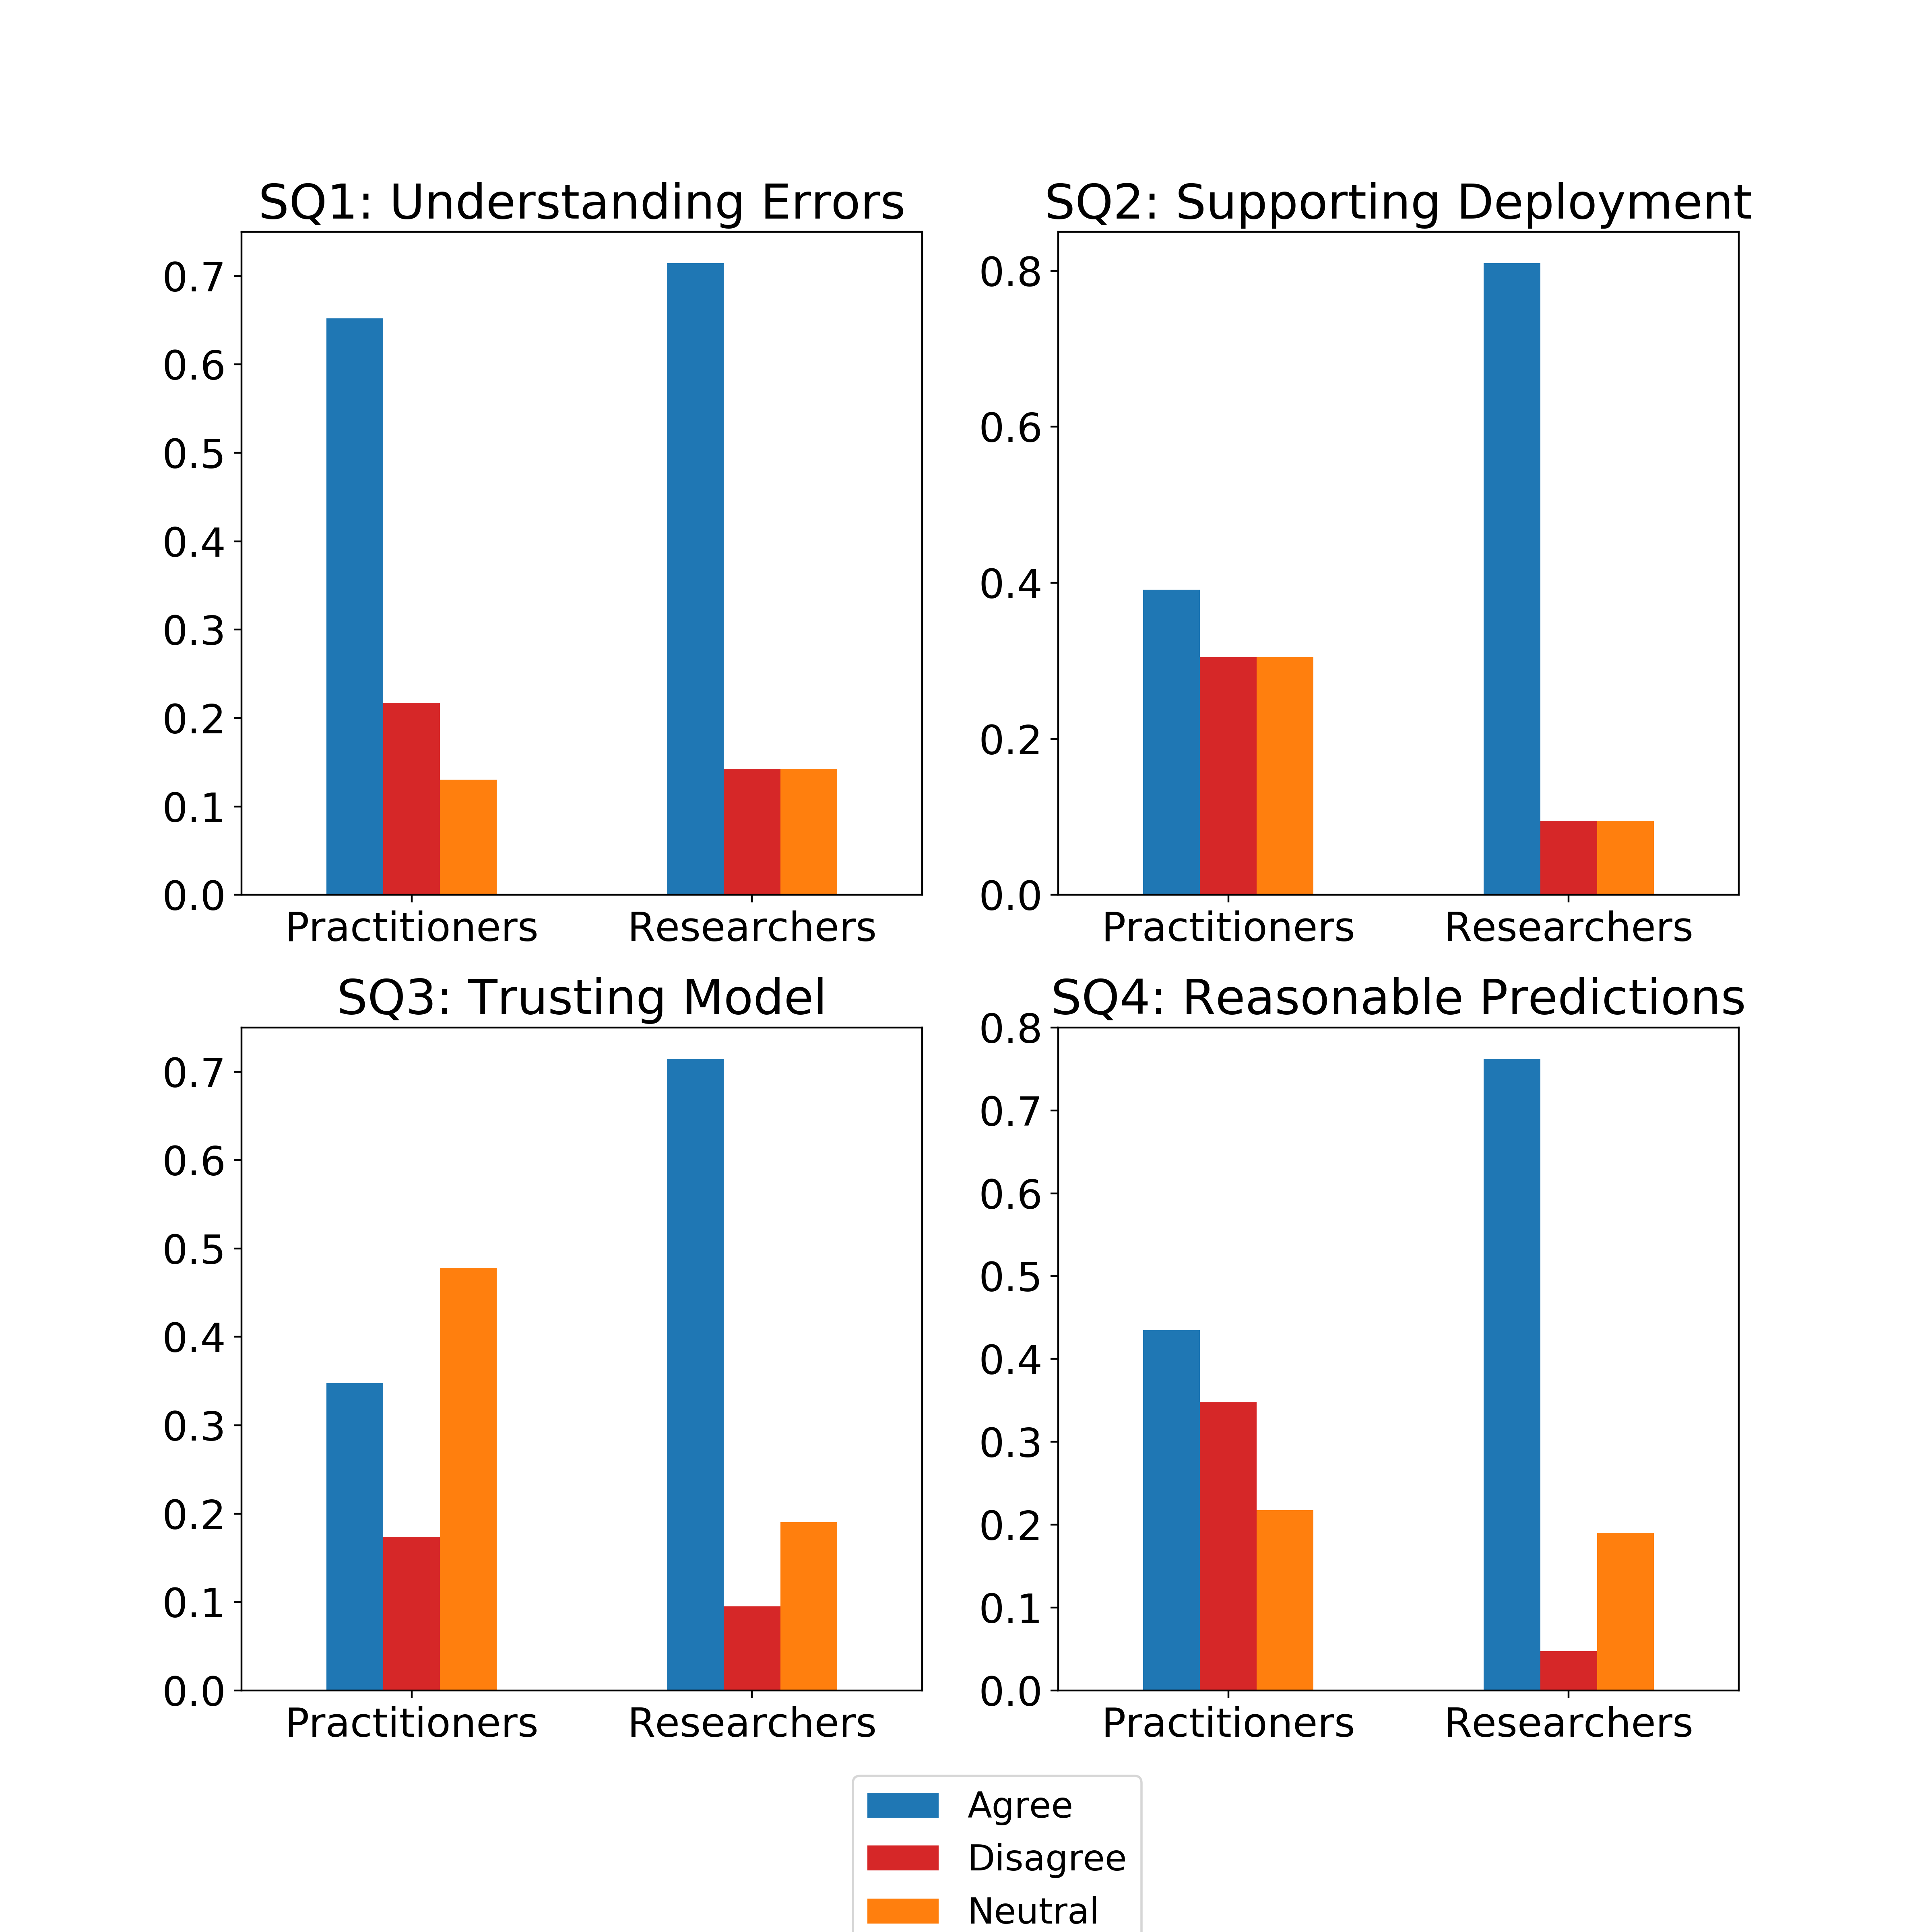
\includegraphics[clip,trim=0mm 0mm 0mm 0mm,scale=0.35]{04-research-mcbrp/academia-vs-industry}
  \caption{Results from a within-subject study comparing answers between participants who are practitioners or researchers (in the treatment group).}
 \label{fig:aca-vs-ind}
\end{figure}

\subsection{Comparing Attitudes in the Treatment Group}
Based on the users who saw the explanations, we compare the distributions of answers between practitioners and researchers in Figure~\ref{fig:aca-vs-ind} in order to understand the needs of different types of users. 
We find that there is a significant difference between practitioners and researchers for SQ2 ($\chi^{2} = 7.94$, $\alpha = 0.05$), indicating that more researchers are in favor of using the model as a forecasting tool, and less are against it or have a neutral attitude, in comparison to the practitioners. 
We also find a significant difference for SQ3 ($\chi^{2} = 5.98$, $\alpha = 0.05$): a larger proportion of researchers trust the model, while the majority of practitioners have neutral feelings. 
The results for SQ4 are significant as well ($\chi^{2} = 6.86$, $\alpha = 0.05$): 
although the majority of users in both groups believe the model produces reasonable predictions, a larger proportion of the practitioners disagree with this statement in comparison to the researchers. 

We see no significant difference between groups for SQ1 ($\chi^{2}$ test, $\alpha = 0.05$), which makes sense given that we showed that \OurMethod{} explanations have a similar effect on both practitioners and researchers when comparing users in the treatment and control groups in Section~\ref{section:conditioning}. 

Overall, these results suggest that our user study population is fairly heterogeneous, and that users from different backgrounds have different criteria for deploying or trusting a model, and varying levels of confidence regarding the accuracy of its outcomes. 


\subsection{User Study Limitations}
Like any user study, ours has some limitations. 
It would have been preferable to distribute users more evenly in terms of the proportion of users in the treatment and control groups, as well as the proportion of practitioners and researchers in each of these groups. 
Unfortunately, this was not possible in our case because we recruited participants in two rounds: first for the treatment group, and then afterwards for the control group. 
One option could be to discard some practitioners in the control group in order to have a better balance in terms of background, but we felt it was more important to have as many users as possible, and it would not be clear how to choose which users to discard. 
Fortunately, we found that our results still hold when conditioning on background as mentioned in Section~\ref{section:conditioning}. 
In future work, we plan to recruit for both groups at the same time to avoid issues like these. 

We also acknowledge that not having a baseline method to compare to is a limitation of our study. 
In our case, the main issue is that there simply does not exist a method that is specifically for explaining errors in regression predictions, which would make asking questions about errors 
\begin{inparaenum}[(i)]
	\item unfair, and 
	\item confusing, as mentioned in Sections~\ref{section:lime} and~\ref{section:studydesign}. 
\end{inparaenum}
However, now that \OurMethod{}  exists, it can serve as a baseline for future work on erroneous predictions, which is another contribution of this paper. 


